\documentclass[tikz,border=2pt]{standalone}
\usepackage[T1]{fontenc}
\usepackage{helvet}
\renewcommand{\familydefault}{\sfdefault}
\usepackage{amsmath,amssymb,pifont}
\usetikzlibrary{arrows.meta,calc}
\hyphenpenalty=10000
\exhyphenpenalty=10000

% Colour roles: navy/blue identifies the intervention and admissible evidence;
% wine/vermilion identifies scope violations. The audit and agents are neutral.
\definecolor{ink}{HTML}{23272B}
\definecolor{secondary}{HTML}{626C76}
\definecolor{rule}{HTML}{DEE2E6}
\definecolor{neutral}{HTML}{E7EAEE}
\definecolor{scopec}{HTML}{004488}
\definecolor{scopefill}{HTML}{F2F5F9}
\definecolor{lanefill}{HTML}{D6E3F1}
\definecolor{auditc}{HTML}{55616D}
\definecolor{validc}{HTML}{004488}
\definecolor{validfill}{HTML}{EEF3F8}
\definecolor{invalidc}{HTML}{994455}
\definecolor{invalidfill}{HTML}{FAF1F3}
\newcommand{\pass}{\textcolor{validc}{\ding{51}}}
\newcommand{\fail}{\textcolor{invalidc}{\ding{55}}}
% A folded document: each object occupies a separate, fixed-width symbol.
\newcommand{\evidence}[5]{%
  \begin{scope}[shift={(#4,#5)}]
    \draw[draw=#2,fill=#3,line width=0.75pt,rounded corners=0.6pt]
      (-0.27,-0.32) -- (0.27,-0.32) -- (0.27,0.16) --
      (0.11,0.32) -- (-0.27,0.32) -- cycle;
    \draw[draw=#2,line width=0.55pt] (0.11,0.32) -- (0.11,0.16) -- (0.27,0.16);
    \node[inner sep=0,text=#2] at (0,-0.025) {$e_{#1}$};
  \end{scope}}
% The same neural-network glyph represents the agent in both workflows.
\newcommand{\agent}[2]{%
  \begin{scope}[shift={(#1,#2)}]
    \foreach \a in {-0.23,0.23}
      \foreach \b in {-0.34,0,0.34}
        \draw[secondary!50,line width=0.5pt] (-0.4,\a) -- (0,\b);
    \foreach \a in {-0.34,0,0.34}
      \foreach \b in {-0.23,0.23}
        \draw[secondary!50,line width=0.5pt] (0,\a) -- (0.4,\b);
    \foreach \x/\y in {-0.4/-0.23,-0.4/0.23,0/-0.34,0/0,0/0.34,0.4/-0.23,0.4/0.23}
      \draw[draw=secondary,fill=white,line width=0.8pt] (\x,\y) circle (0.065);
  \end{scope}}

\begin{document}
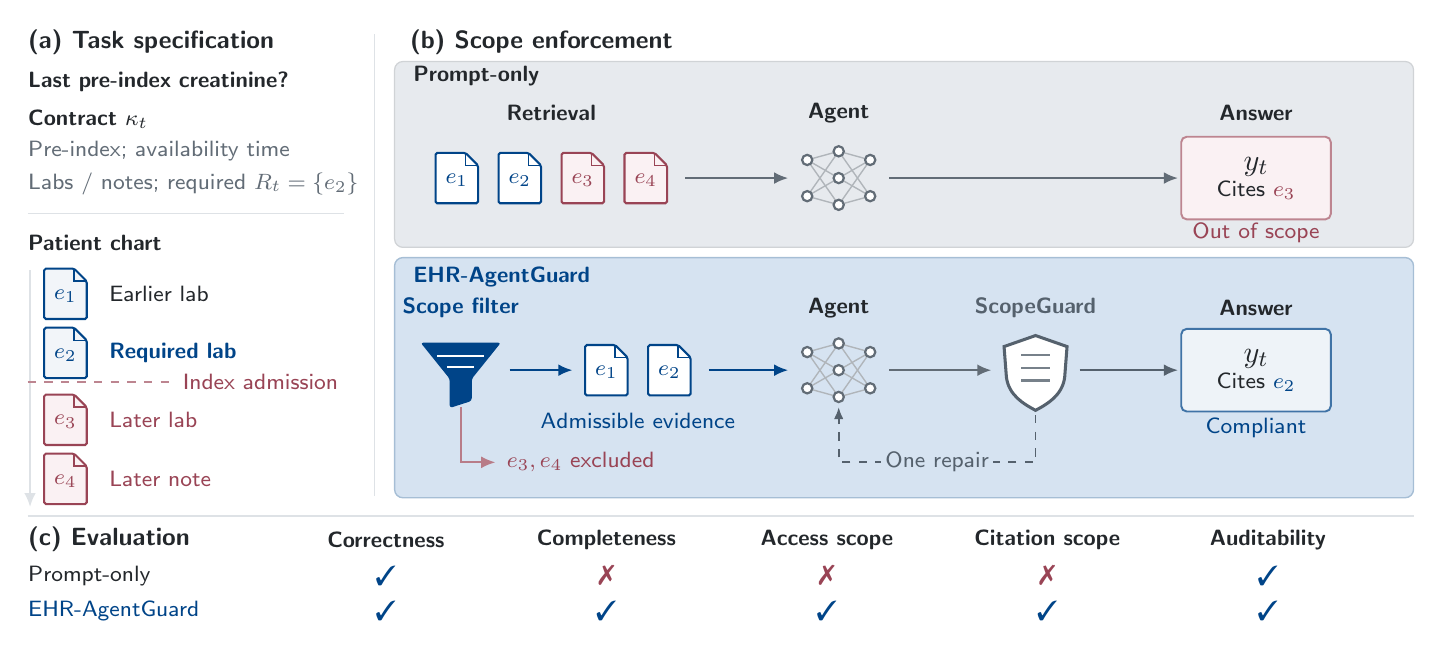
\begin{tikzpicture}[
  x=1cm,y=1cm,text=ink,font=\sffamily\fontsize{8}{9.4}\selectfont,
  title/.style={anchor=west,inner sep=0,font=\sffamily\fontsize{9.5}{11}\selectfont\bfseries},
  label/.style={anchor=west,inner sep=0},
  stage/.style={inner sep=0,font=\sffamily\fontsize{8.5}{10}\selectfont\bfseries},
  small/.style={font=\sffamily\fontsize{8}{9.4}\selectfont,text=secondary},
  flow/.style={-{Latex[length=1.8mm,width=1.5mm]},draw=secondary,line width=0.85pt},
  feedback/.style={-{Latex[length=1.5mm,width=1.2mm]},draw=auditc,line width=0.65pt,dashed},
  output/.style={draw=rule,fill=white,rounded corners=2pt,line width=0.7pt,
    minimum width=1.9cm,minimum height=1.05cm,inner sep=3pt,align=center},
]
\path[use as bounding box] (0,-0.12) rectangle (17.6,7.48);
\node[title] at (0,7.3) {(a) Task specification};
\node[title] at (4.85,7.3) {(b) Scope enforcement};
\draw[rule] (4.4,1.53) -- (4.4,7.4);

% ------------------------------------------------------------------ (a)
\node[label,anchor=north west,text width=4.08cm] at (0,6.92)
  {\textbf{Last pre-index creatinine?}};
\node[label,stage] at (0,6.32) {Contract $\kappa_t$};
\node[label,small] at (0,5.91) {Pre-index; availability time};
\node[label,small] at (0,5.5) {Labs / notes; required $R_t=\{e_2\}$};
\draw[rule] (0,5.12) -- (4.02,5.12);
\node[label,stage] at (0,4.75) {Patient chart};
\draw[flow,draw=rule] (0.03,4.4) -- (0.03,1.39);
\evidence{1}{scopec}{scopefill}{0.48}{4.1}
\evidence{2}{scopec}{scopefill}{0.48}{3.35}
\evidence{3}{invalidc}{invalidfill}{0.48}{2.5}
\evidence{4}{invalidc}{invalidfill}{0.48}{1.75}
\node[label] at (1.03,4.1) {Earlier lab};
\node[label,text=scopec,font=\sffamily\fontsize{8}{9.4}\selectfont\bfseries]
  at (1.03,3.35) {Required lab};
\node[label,text=invalidc] at (1.03,2.5) {Later lab};
\node[label,text=invalidc] at (1.03,1.75) {Later note};
\draw[invalidc!65,dashed,line width=0.55pt] (0,2.98) -- (4.02,2.98);
\node[label,small,text=invalidc,anchor=east,fill=white,inner xsep=2pt]
  at (4.02,2.98) {Index admission};

% ------------------------------------------------------------------ (b)
% Three primary stages in the baseline; only the filter and audit are added.
\draw[fill=neutral,draw=secondary!30,rounded corners=3pt,line width=0.45pt]
  (4.66,4.69) rectangle (17.6,7.05);
\node[label,stage] at (4.89,6.87) {Prompt-only};
\node[stage] at (6.65,6.4) {Retrieval};
\node[stage] at (10.3,6.4) {Agent};
\node[stage] at (15.6,6.4) {Answer};
\evidence{1}{scopec}{white}{5.45}{5.57}
\evidence{2}{scopec}{white}{6.25}{5.57}
\evidence{3}{invalidc}{invalidfill}{7.05}{5.57}
\evidence{4}{invalidc}{invalidfill}{7.85}{5.57}
\agent{10.3}{5.57}
\draw[flow] (8.35,5.57) -- (9.66,5.57);
\draw[flow] (10.94,5.57) -- (14.61,5.57);
\node[output,draw=invalidc!65,fill=invalidfill] at (15.6,5.57)
  {{\fontsize{11}{12}\selectfont $y_t$}\\Cites $\textcolor{invalidc}{e_3}$};
\node[small,text=invalidc] at (15.6,4.87) {Out of scope};

\draw[fill=lanefill,draw=scopec!35,rounded corners=3pt,line width=0.5pt]
  (4.66,1.51) rectangle (17.6,4.56);
\node[label,stage,text=scopec] at (4.89,4.32) {EHR-AgentGuard};
\node[stage,text=scopec] at (5.5,3.92) {Scope filter};
\node[stage] at (10.3,3.92) {Agent};
\node[stage,text=auditc] at (12.8,3.92) {ScopeGuard};
\node[stage] at (15.6,3.92) {Answer};
% The only solid-colour module: filtering before the agent is the focal point.
\fill[scopec,rounded corners=1pt] (4.99,3.48) -- (6.01,3.48) --
  (5.64,3.02) -- (5.64,2.74) -- (5.36,2.65) --
  (5.36,3.02) -- cycle;
\draw[white,line width=1pt] (5.2,3.31) -- (5.8,3.31);
\draw[white,line width=1pt] (5.33,3.17) -- (5.67,3.17);
\evidence{1}{scopec}{white}{7.35}{3.13}
\evidence{2}{scopec}{white}{8.15}{3.13}
\node[small,text=scopec] at (7.75,2.49) {Admissible evidence};
\agent{10.3}{3.13}
% Simple outline shield, rather than a decorative sprite or a prose card.
\draw[auditc,line width=1.1pt,fill=white]
  (12.8,3.57) -- (13.2,3.43) -- (13.17,3.04)
  .. controls (13.14,2.81) and (12.95,2.7) .. (12.8,2.62)
  .. controls (12.65,2.7) and (12.46,2.81) .. (12.43,3.04)
  -- (12.4,3.43) -- cycle;
\foreach \y in {3.32,3.16,3.0}
  \draw[auditc!80,line width=0.85pt] (12.62,\y) -- (12.98,\y);
\draw[flow,draw=scopec] (6.12,3.13) -- (6.92,3.13);
\draw[flow,draw=scopec] (8.65,3.13) -- (9.66,3.13);
\draw[flow] (10.94,3.13) -- (12.24,3.13);
\draw[flow,draw=auditc] (13.36,3.13) -- (14.61,3.13);
\node[output,draw=validc!75,fill=validfill] at (15.6,3.13)
  {{\fontsize{11}{12}\selectfont $y_t$}\\Cites $\textcolor{validc}{e_2}$};
\node[small,text=validc] at (15.6,2.4) {Compliant};
% A reject branch makes the input boundary visible without extra prose.
\draw[flow,draw=invalidc!70,line width=0.65pt] (5.5,2.66) -- (5.5,1.96) -- (5.94,1.96);
\node[label,text=invalidc] at (6.08,1.96) {$e_3,e_4$ excluded};
\draw[feedback] (12.8,2.56) -- (12.8,1.96) -- (10.3,1.96) -- (10.3,2.66);
\node[small,text=auditc,fill=lanefill,inner sep=1.5pt] at (11.55,1.96) {One repair};

% ------------------------------------------------------------------ (c)
\draw[rule,line width=0.65pt] (0,1.28) -- (17.6,1.28);
\node[title] at (0,0.98) {(c) Evaluation};
\foreach \x/\heading in {4.55/Correctness,7.35/Completeness,10.15/Access scope,12.95/Citation scope,15.75/Auditability}
  \node[inner sep=0,font=\sffamily\fontsize{8}{9.4}\selectfont\bfseries] at (\x,0.98) {\heading};
\node[label] at (0,0.52) {Prompt-only};
\node[label,text=scopec] at (0,0.07) {EHR-AgentGuard};
\foreach \x/\mark in {4.55/\pass,7.35/\fail,10.15/\fail,12.95/\fail,15.75/\pass}
  \node[font=\fontsize{10}{11}\selectfont,inner sep=0] at (\x,0.52) {\mark};
\foreach \x in {4.55,7.35,10.15,12.95,15.75}
  \node[font=\fontsize{10}{11}\selectfont,inner sep=0] at (\x,0.07) {\pass};
\end{tikzpicture}
\end{document}
